% Fig. scoring (b): drainage test on a hemispherical bowl profile (radius 0.9 cm), side view.
% Upright bowl = arc from 180 to 360 deg; a tilt of phi rotates it to 180+phi .. 360+phi.
% phi = 56: rim ends at 236 and 56 deg, bottom (270) is on the arc, so water fills the
%           circular segment below the chord at z = 0.9 sin(236) (from 236 to 304 deg).
% phi = 135: arc 315 .. 495 deg; its lowest point is the rim end at 315 deg, so it drains.
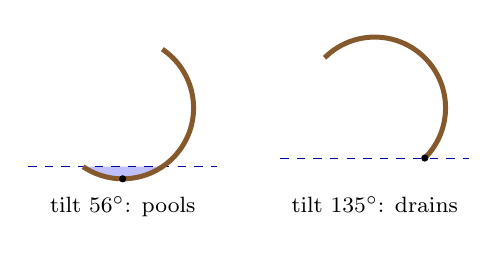
\begin{tikzpicture}[x=1cm,y=1cm,font=\footnotesize]
  \begin{scope}
    \fill[blue!25] (236:0.9) arc[start angle=236,end angle=304,radius=0.9] -- cycle;
    \draw[blue!60!black,dashed] (-1.2,{0.9*sin(236)}) -- (1.2,{0.9*sin(236)});
    \draw[line width=1.8pt,brown!70!black] (236:0.9) arc[start angle=236,end angle=416,radius=0.9];
    \fill (270:0.9) circle (1.3pt);
    \node[anchor=north,align=center] at (0,-1.0) {tilt $56^\circ$: pools};
  \end{scope}
  \begin{scope}[xshift=3.2cm]
    \draw[blue!60!black,dashed] (-1.2,{0.9*sin(315)}) -- (1.2,{0.9*sin(315)});
    \draw[line width=1.8pt,brown!70!black] (315:0.9) arc[start angle=315,end angle=495,radius=0.9];
    \fill (315:0.9) circle (1.3pt);
    \node[anchor=north,align=center] at (0,-1.0) {tilt $135^\circ$: drains};
  \end{scope}
\end{tikzpicture}
